 \documentclass[10pt,a4paper]{article}
\usepackage[T1]{fontenc}
\usepackage[utf8]{inputenc}
\usepackage[brazil]{babel}
\usepackage{indentfirst}
\usepackage{graphicx}
\usepackage[section]{placeins}

\begin{document}

	\title{INF01124 - Classificação e Pesquisa de Dados - Exercício 3}
	\date{}
	\author{Felipe de Almeida Graeff\\00261606}
	\maketitle

	\section{Hybrid Sort}

		\begin{enumerate}

			\item Após rodar o algoritmo implementado, foi constatado que existem
      961 pares de chaves e cadeados, como pode ser conferido na saída do
      programa mostrada a seguir.

      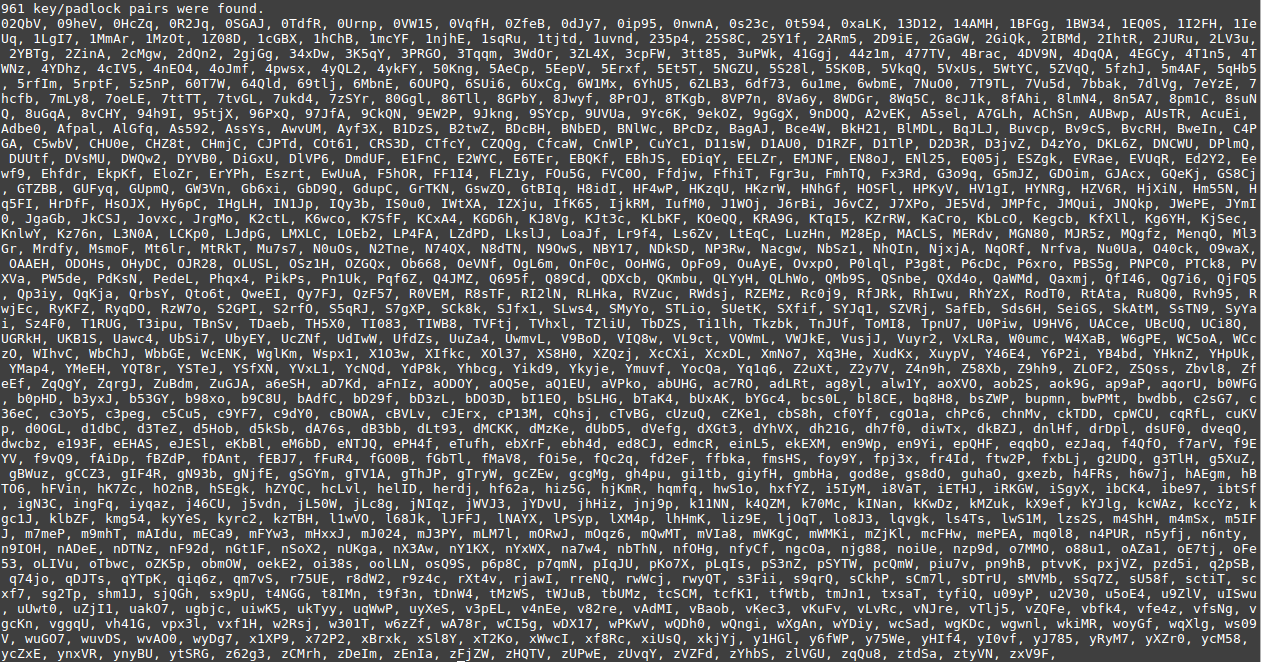
\includegraphics[width=\textwidth]{keys.png}

			\item A seguintes tabelas contém as estatísticas pedidas.

        {\large Lista de chaves}

        \begin{tabular}{ r | c }
          Total de \emph{swaps}           & $5146$    \\  \hline
          Total de chamadas recursivas    & $1307$    \\  \hline
          Maior razão de particionamento  & $979$     \\  \hline
          Menor razão de particionamento  & $1$       \\  \hline
          Razão de particionamento média  & $16.4273$ \\
        \end{tabular}


        {\large Lista de cadeados}

        \begin{tabular}{ r | c }
          Total de \emph{swaps}           & $5929$    \\  \hline
          Total de chamadas recursivas    & $1293$    \\  \hline
          Maior razão de particionamento  & $979$     \\  \hline
          Menor razão de particionamento  & $1$       \\  \hline
          Razão de particionamento média  & $16.2368$ \\
        \end{tabular}

      \item Comparação de tempo de execução utilizando particionamento constante
      e particionamento aleatório.

        \begin{tabular}{ r | c | c |}
                              & Lista de chaves & Lista de cadeados \\ \hline
          Quicksort padrão    & $0.000841s$     & $0.000823s$       \\ \hline
          Quicksort aleatório & $0.000874s$     & $0.000896s$       \\ \hline
        \end{tabular}

		\end{enumerate}

		
	\section{Radix Sort}
	
\end{document}
